%% example.tex
%% Jeremy Singer
%% 16 Oct 12

\documentclass{mpaper}

\usepackage{algorithm2e}
\usepackage [english]{babel}
\usepackage [autostyle, english = american]{csquotes}
\MakeOuterQuote{"}

\begin{document}

\title{Improving the speed and accuracy of phylogenetic tree construction using deep reinforcement learning}
\author{Paul Bekaert}
\matricnum{2517073B}

\maketitle

\begin{abstract}    
A phylogenetic tree is a diagram which shows how living species relate to one another, and is an essential tool in research to determine biological patterns. This can be useful for finding the evolutionary traits of a species and classifying them. Construction of such trees is complex and difficult to scale, and the most accurate methods usually compromise speed for accuracy. However, the use of neural networks to speed up the search of these trees has just scratched the surface. In this paper, we explore the use of GNNs and deep neural networks to accelerate the process. Our results show that it is possible to find phylogenetic trees in linear time, O(n), and is more scalable than other methods such as RAxML-NG. However, it was not able to achieve the same level of log likelihood as such methods, with on average a log likelihood result 20\% less than RAxML-NG. We conclude the paper with the determination that deep neural networks are likely a viable way to accelerate the speed of phylogenetic tree construction, whilst GNNs are less effective. Future research could include the use of the MCTS (Monte Carlo Tree Search) algorithm to improve accuracy, and expand network training to work for other substitution matricies.
\end{abstract}

% \begin{enumerate}
% \item General description of the problem, motivation, relevance
% \item Background information, possibly including a literature survey
% \item Description of approach taken to solve the problem, including
%   high-level design and lower-level implementation details as appropriate
% \item Evaluation, qualitative or quantitative as appropriate
% \item Conclusion, including scope for future work
% \end{enumerate}

\section{Introduction}

\subsection{Phylogenetic Trees}

In biology, phylogenetics is the study of relationships among groups of species which form due to evolution. Phylogenetic trees are dendrograms (a diagram where the branch length expresses similarity between clusters, see Figure 1) used by researchers to classify and visualize the "distance" between species. They represent taxa, which are clusters of species. Different attributes can be used to organise phylogenetic trees, however the focus of this research will be proteins. They are found by comparing the differences between the same amino acid chain (protein) in different species, and finding similarities between them. Amino acid chains are derived from nucleotide sequences, where groups of three nucleotides (codons) correspond to particular amino acids. Due to the possibility of silent mutations in nucleotide sequences - when a change in one nucleotide does not change the protein - we favour the use of amino acid chains, as they are less noisy given our dataset. Nevertheless, amino acid chains still retain enough information to infer relationships between proteins. Depending on the method used and quality of the tree desired, creating accurate phylogenetic trees can be at worst NP-hard.

\begin{figure}[h]
    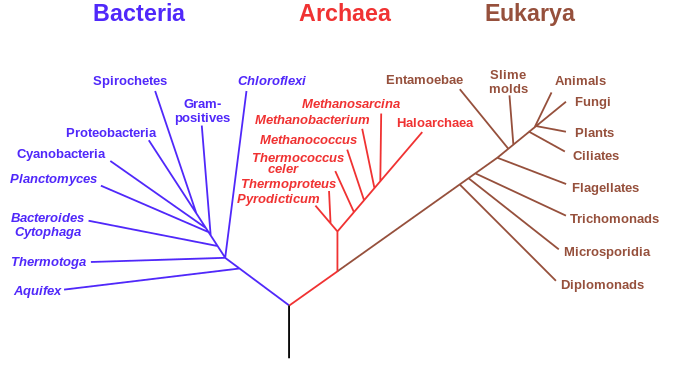
\includegraphics[width=1\linewidth]{images/Phylogenetic_tree_example}
    \centering
    \caption{An example of a phylogenetic tree \cite{enwiki:1187886462}.}
\end{figure}

Phylogenetic trees consist of taxa and clades. Clades are the "glue" of different taxa and other clades. Since the trees do not have "in-between" nodes (all the taxa are leaf nodes), the clades create the connections between different groups of taxa. They can behave as regular graph nodes, and be restructured in different ways.

\subsection{Tree Operations}

For a tree that has already been constructed, a singular operation called subtree pruning and regrafting (SPR) can be used to edit the tree. An SPR operation is one which restructures a phylogenetic tree by moving one sub-branch to another part of the tree. The operation is complete, which means any possible tree can be constructed from any tree via repeatedly applying this operation \cite{semple2003phylogenetics}. It's important that after the operation has completed, that there are no "unifurcations" - clades which connect to only one other clade. This can be removed by changing the ordering of the pointers. Figure 2 demonstrates an SPR operation. A branch is selected, and "pruned" from the tree. This creates two separate trees, which can then be joined together with a new branch. In this example, the taxa in clade $CDE$ was deemed more similar to $H$ than $F$, and therefore regrafted in such a way that it links closer to $H$. This operation is covered here as it is widely used in phylogenetic algorithms.

% FIX THE FIGURE ALMOST OVERLAPPING TEXT

\begin{figure}[h]
    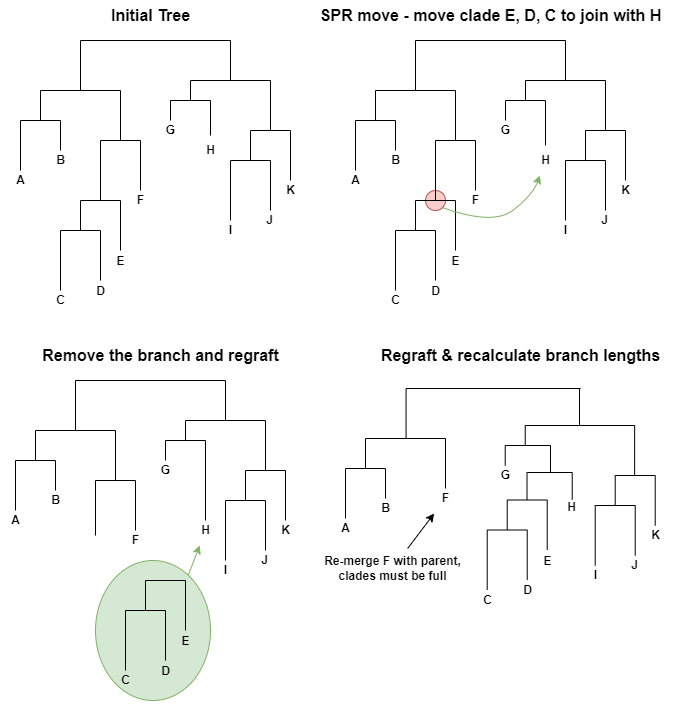
\includegraphics[width=1\linewidth]{dissertation/images/spr_example.png}
    \centering
    \caption{An example SPR operation. Clade CDE was deemed to be closer to taxa H than F. A branch optimization algorithm is run after the move has completed.
    }
\end{figure}

\subsection{Deep Learning}

Most methods that have been used to generate phylogenetic trees are based on algorithmic or probabilistic models. Given the complexity of the problem, deep learning seems to be a viable approach to build them. The two main types of deep learning which will be used in this research are deep reinforcement learning and graph neural networks. Reinforcement learning treats the problem as a game, trying to optimize the end result score by taking a set of actions in a sequence. Deep reinforcement learning is a method used to teach agents how to navigate an action space by actions they can take. For example, an AI playing a game of Tetris will use deep reinforcement learning to decide which placement of the blocks will lead to the best outcome \cite{stevens2016playing}. The reward at the end of the game informs the AI whether they have played well or not (in Tetris, this would be the final score). The AI then learns from the result by adapting its behaviour to maximise the score. Graph Neural Networks (GNNs) are a different type of neural network. They explore graph structures and give an overall score to a graph. They can also be used in a convolutional sense. Graph Convolutional Neural Networks (GCNNs) explore graphs and attribute properties to nodes that depend on their neighbour's nodes. 

There are several different types of Graph Neural Networks \cite{Sanchez2021}. Graph prediction assesses the graph as a whole and gives a singular output. GNNs of this type are often useful for classification, or extrapolating key graph features. Edge-level GNNs give outputs for only the edges in the graph. They are useful for quantifying the importance of certain edges, and finding attributes about relationships between elements. Among other uses, they can be tasked to create new edges (link prediction), edge weight prediction, or edge classification. Node-level prediction is when the GNN gives a score to each node. Each node in the graph is given a value based off its neighbours (which are joined by edges). They can be used to calculate node attributes, and classify nodes. Furthermore, node-level GCNNs can classify nodes based off a convolution which can be several neighbours deep.

\vspace{3cm}

\subsection{Summary}

This section examines the basics of phylogenetic trees, starting with their definition: diagrams showing the evolutionary clustering of different taxa. In this research, they are built based on amino acid sequences, as they have less noise than nucleotide sequences for the taxa we will be working with. We then explored the main operation which can be performed on such trees: the SPR operation. SPR moves consist of pruning one part of the tree and re-attaching it someplace else in a way that does not leave any hanging unifurcations. Finally, different types of GNNs were discussed: graph-level, edge-level, and node-level. GCNNs are a type of network which can encompass all three methods, but are different to GNNs as they convolute over the node neighbours.

\section{Background}

\subsection{Algorithmic Methods}

Algorithmic methods to construct phylogenetic trees are split into two main groups, each having their pros and cons. The first one is UPGMA (Unweighted Pair Group Method Arithmetic Mean) introduced by Sneath et al. \cite{sneath1973numerical} in 1973. UPGMA builds rooted phylogenetic trees using a distance matrix between amino acids. There are many different distance matrix generation methods, and one such model is BLOSUM 62. UPGMA works by identifying the two species with the shortest distance (calculated using the distance matrix and amino acid chains) at every iteration, joining them, and then comparing the distance of each species with the newly formed group. Although a fast and easy algorithm to implement, UPGMA  has the crucial flaw of assuming a constant rate of evolution \cite{melnick11985genetic}. Different species have different rates of evolution, and therefore this assumption of a constant rate of evolution cannot hold true to create accurate trees. 

The second well-known method in algorithmic reconstruction of phylogenetic trees is neighbour join, first pioneered by Saitou et al. \cite{njpaper}. This method creates unrooted trees, unlike UPGMA. Instead of joining the two species with the lowest distance between each other, it does a normalization of the overall tree to get the smallest overall branch lengths over the entire tree. Using this method, neighbour join does not assume a constant rate of evolution and may be a better choice if one cannot assume that their lineages will have a constant rate of evolution. Although this method is generally more accurate, it is slower than UPGMA. The main drawback of both methods is that they are relatively inaccurate, and still tend to slow down with larger datasets.

% DESCRIBE WHAT ARE SEQUENCE PROFILES?
FastTree, developed by Price et al. \cite{fasttree1}, revolutionised phylogenetic tree building. Due to limitations in computing power in 2009, it was considered difficult to scale algorithms for inferring phylogenies with over 10,000 alignments \cite{fasttree1}. FastTree leveraged sequence profiles instead of an amino acid distance table, which reduced the complexity from O($n^2$) using traditional methods such as UPGMA, to O($n\sqrt{n} \log{(n)}$). The method revolved around distance vectors which were calculated based on the nodes' children. An initial unrooted tree is constructed, with all children connected to each other in a star formation. From there, only SPR moves are used to improve the tree. The distance between two nodes' vectors was the distance used to calculate the tree. A heuristic function was also used to reduce the amount of possible SPR operations from $O(n^{3})$ to $O(n\log n)$, speeding up the algorithm. In essence, it is a neighbour-joining method which uses sequence profiles instead of entire sequences to make comparisons faster, and uses said heuristic function to narrow the search. It is a lot more scalable and efficient than both UPGMA and neighbour join, as it does not need a distance matrix. However, it is known to be sensitive to the initial evolutionary assumptions, and the statistical assumptions used for the profile vectors are not complex enough to properly represent them, which can lead to errors in the output. Though it has its misgivings, it is considered to be better than both UPGMA and other conventional neighbour join methods.

\subsection{Maximum Likelihood estimation}

Maximum likelihood estimation (MLE) revolves around the use of models and their parameters to maximise the likelihood of the generated tree \cite{felsenstein1981evolutionary} and is said to be NP-Hard. Aligned amino acids from proteins are used as input to the algorithm, which then uses a selected model to create an evolutionary tree of said proteins. With this tree, a phylogenetic tree of the organisms containing the proteins can be inferred. Next, it will use a likelihood calculation on the tree. The likelihood value is the probability that a given tree would generate the existing sequence data, meaning that the higher the likelihood, the better the tree. This value is used to tweak the parameters of the model to try and optimize said likelihood. Depending on the algorithm, the parameter space is improved upon. One example is a stochastic hill climbing algorithm searching the parameter space with the help of a regression to find the optimal parameters \cite{nguyen2015iq}. Once the algorithm can no longer improve the likelihood, the tree is returned. Essentially, different trees are searched until the best one (maximum likelihood) is found. There are many models, and well-known ones include Jukes-Cantor \cite{erickson2010jukes}, Kimura models (reductions of Jukes-Cantor) \cite{huelsenbeck1995performance}, and Bayesian models \cite{bollback2002bayesian}. The main advantage of a likelihood model is its accuracy, as it has been proved to create much better trees than other algorithmic methods \cite{fasttree2}. However, it is inherently slow, and becomes incomputable for larger amounts of taxa due to the branching factor and likelihood calculation. Researchers have been trying to accelerate the likelihood calculation by estimating it, bootstrapping, or using various other techniques.

Felsenstein et al. \cite{felsenstein1981evolutionary} were the first to pioneer maximum likelihood in a computational sense, with their algorithm, F84. It was a basic concept of tree likelihood, and has two parameters representing different rates of evolution of nucleotides. Although a limited software, it was what inspired their next software, PHYLIP. PHYLIP \cite{felsenstein1993phylip} uses more advanced substitution models for evolution and was widely used as the foundation for subsequent maximum likelihood methods. A heuristic tree search is employed to explore a large number of actions (such as neighbour joining or SPR) and topologies in an efficient manner. 

First built in 2003, RAxML-NG is a well-known algorithm and tool to compute trees based on maximum likelihood estimation \cite{kozlov2019raxml}. Using MSAs, a substitution model is defined that describes how amino acid substitutions develop over time. Like typical MLE algorithms, RAxML will search for the tree that maximises the likelihood given the sequence data under the chosen substitution model. RAxML is optimized for large scale data through parallelization, and is able to handle hundreds of thousands of sequences whilst still providing a high degree of accuracy.

Whilst FastTree was an innovative paper which advanced the search of phylogenetic trees, it has proved to be less accurate than maximum likelihood approaches. Price et al. acknowledge this in their FastTree 2 paper \cite{fasttree2}, which improves upon the first algorithm by leveraging maximum likelihood. SPR and NNI (Nearest Neighbour Interchange) operations are used to modify the phylogenetic tree and improve its likelihood. To speed up the maximum likelihood, they use the same heuristics to strike a balance between the best likelihood possible and speed. With these heuristics, they are able to reduce the number of SPR actions from $O(n^2)$ to $O(n)$, using two rounds of linear SPR (a limitation which allows branches to only move as far as a certain radius $r$). Thanks to its optimizations, it can handle alignments with hundreds of thousands of taxa in a short amount of time while still being more accurate than UPGMA or Neighbour Join.

To make this literature review comprehensive, we will also cover two more widely used MLE methods. IQ-Tree \cite{nguyen2015iq} is a well known heuristic and model based search, which uses a phylogenetic model selection process to find the most appropriate model for the data at hand. An ultra-bootstrap method is employed, speeding up reliable results. Bootstrapping is a method of re-creating the tree many times, and finding connections that re-appear consistently between different versions, ensuring only the most robust connections are used. Genetic algorithms for phylogenetic tree constructions are also used. An example of one is the Genetic Algorithm for Rapid Likelihood Inference (GARLI) \cite{Evolution_and_Genomics_2016}. 
% It is often used for large datasets, and is especially useful in high-throughput sequencing. It can quickly calculate the maximum likelihood tree, though can struggle with more complex phylogenies.

\subsection{Machine Learning}

Machine learning for phylogenetic tree construction has been explored by multiple authors. Liptak et al. \cite{liptak2021constructing} created a reinforcement learning Q-table to predict and fix the distance table in unrooted trees. Although their results were promising, achieving high accuracy in the reconstruction of the original distance matrix, there are a few issues with the paper. The first is they work with training data which was created by the UPGMA tree. Therefore, the RL network can only get as good as the UPGMA algorithm, severely limiting its potential. The second problem is that of branch lengths, as only the topology of the tree is considered. Since only the distance matrix is modified so that UPGMA can re-create the tree, the lengths are not properly considered. This leads to inaccuracies in the clustering, and does not create a reliable result. 

In one paper, an attention model is used to create phylogenetic trees. Zhu et al. \cite{zhu2021applying} attempt to create a circular ordering using said attention model, followed by tree reconstruction using Yushmanov's algorithm \cite{yushmanov1984construction}. The method starts by creating K-mers frequency vectors for each of the sequences, for which the Euclidean distance is defined as the tree metric. An encoder-decoder multi-attention layer model then processes the sequences, outputting a circular ordering. The neural network's reward function depends on both the circular ordering obtained by the decoder and the corresponding length of the tree. Finally, an adaptation of Yushmanov's algorithm uses the K-mer frequency matrix and tree metric to reconstruct a binary X tree, from which a phylogenetic tree can be built. The method does not require MSAs, which expedites the tree creation process as there is no alignment algorithm needed. Although the algorithm was found to produce better trees than UPGMA, it still fell short of some other methods such as neighbour join and MLE. However, it was substantially faster than MLE methods, and therefore concludes that machine learning may be a viable method to create phylogenetic trees that scale to large datasets \cite{zhu2021applying}. 

Azouri et al. \cite{bioMLPaper} worked on testing whether machine learning can be used to learn which SPR action will lead to the tree with the largest resulting likelihood, without having to do the actual calculation. To do this, they calculate the log likelihood of the tree before and after an SPR operation, and they store features of the action which led to the change in log likelihood. A random forest regression uses features of the SPR operation to predict the change in likelihood, and therefore if the move should be performed or not. This method does not use the sequence data, but rather the properties of the current tree and SPR operation.

\begin{figure}
    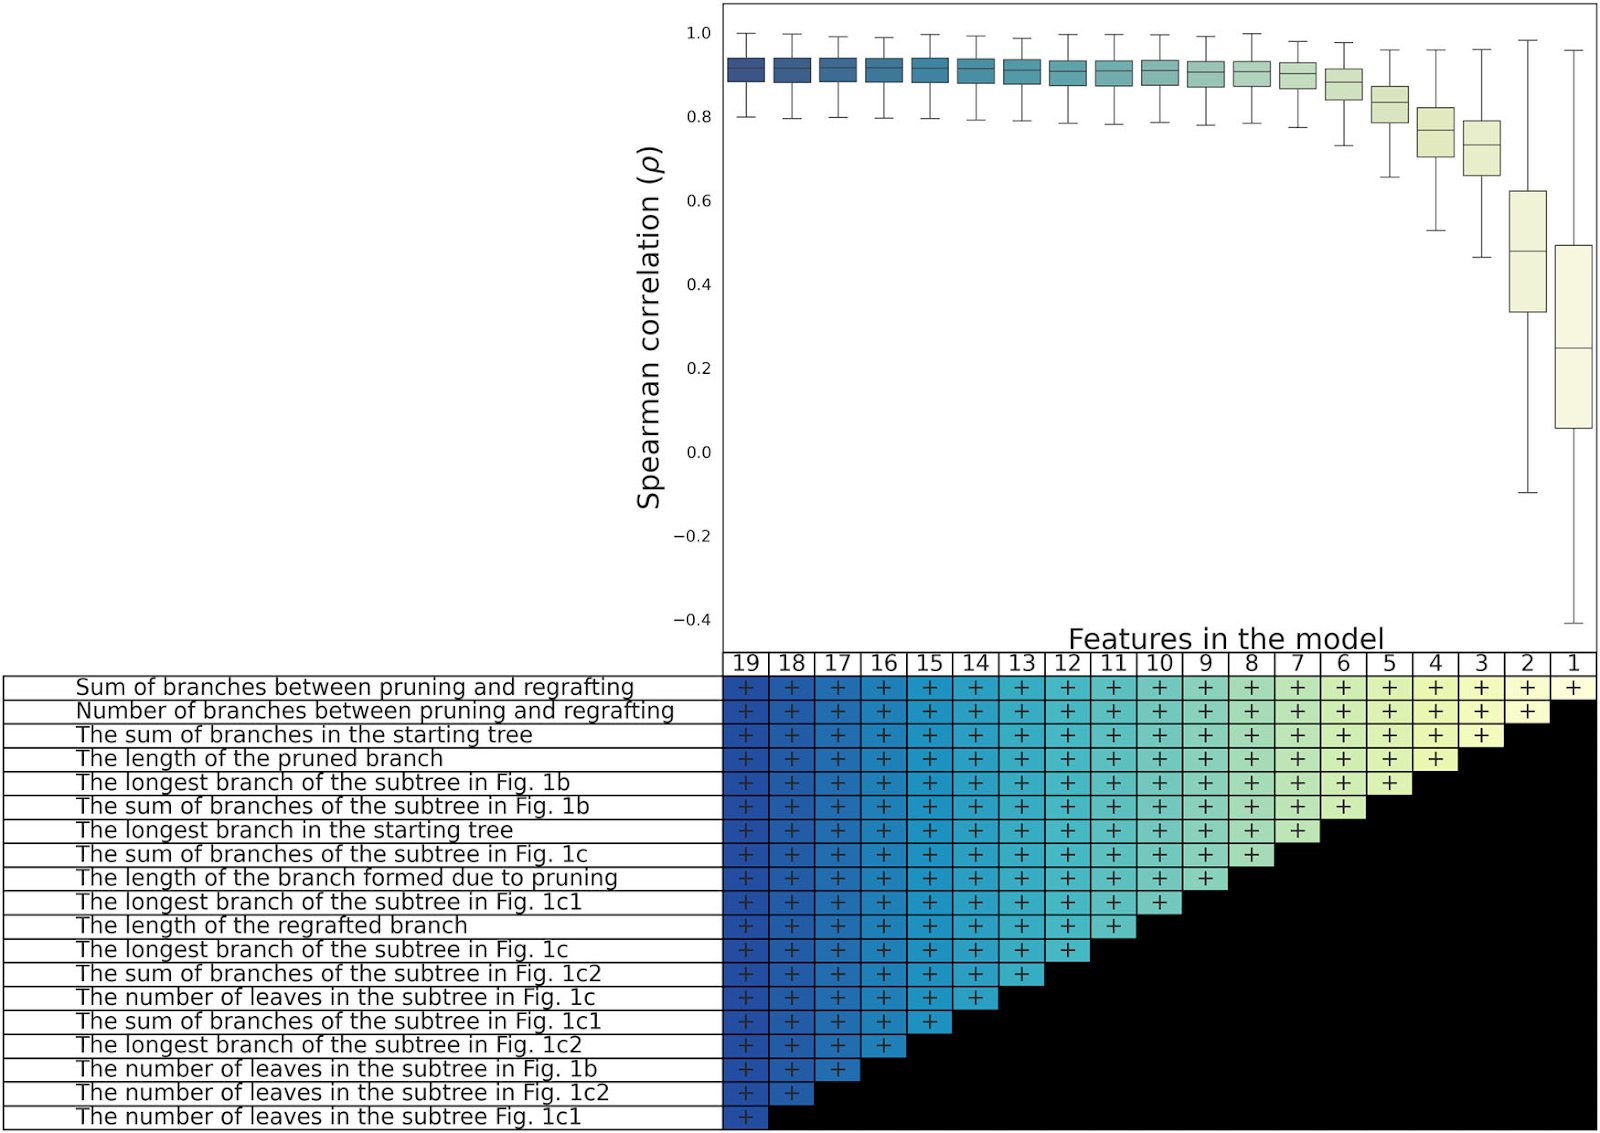
\includegraphics[width=1\linewidth]{dissertation/images/spearman_azouri_biomlpaper.png}
    \centering
    \caption{Spearman's correlation found between the SPR move properties and importance to classification by Azouri et al. \cite{bioMLPaper}. For example, in this diagram, it can be said that the sum of branches between pruning and regrafting was an important feature.}
\end{figure}

Quoting from their paper: "In 81\% and 95\% of the datasets, the best move was among the top 10\% and 25\% predictions, respectively" \cite{bioMLPaper}. This seems to suggest that a machine learning approach to tree reconstruction has potential. However, it could be that the high accuracy was due to the testing data, which may be biased compared to other benchmarking methods such as Rose. A random forest methodology was informative as it can be shown which features were the most effective at differentiating a good action from a bad one. The properties are those of the tree and sub-tree being regrafted, and not of the taxa on the tree (for example, total tree length, sum of nodes, or longest branch in a subtree). A Spearman's correlation is then performed on the properties to find those that were most impactful, shown in Figure 3. It was found that the sum of branches between pruning and regrafting, the number of branches between pruning and regrafting, and other similar features had the greatest effect on finding the correct action. 

% show that the techniques were more limited?
Although Azouri et al. created a working neural network to predict which action would maximise log likelihood, it wasn't until she extended her work by writing "The tree reconstruction game: phylogenetic reconstruction using reinforcement learning" \cite{azouri2023tree} that tree construction using ML was explored further. In that paper, a DQN (Deep Q Network) is used to predict the quality of an SPR action given a phylogenetic tree. The utility function aims at maximising the likelihood of the resulting tree, which is trained using a discount factor to account for future moves. When 7 sequences were used, an accuracy of 99.999\% was found, and with MSAs of 12 sequences, an accuracy of 96.9\%. To deal with a larger number of sequences, restrictions were set on the number of SPR moves, notably considering only local changes in the tree topology. This is determined by a radius, which restricts the SPR move possibilities to only branches within its radius range, limiting SPR moves to a linear amount. With the smaller set of SPR actions, an accuracy of 99.9\% was attained with 15 sequences, suggesting that narrowing the action space is a viable technique for ML and phylogenetic tree construction without hindering accuracy. However, when the number of MSAs increased to 20, the accuracy dropped to 89\%. Azouri et al. speculated that alternative data collection methodologies could be used to increase the accuracy given more sequences, and that 20 is the current limitation for accurate tree generation using their algorithm.

There has been little exploration of the use of GNNs in phylogenetic tree construction. Gaofeng Pan \cite{pan2022graph} is the first to use GNNs for this task. In his paper, he describes using multi-subcellular localization in conjunction with median genome prediction to generate tree topology. Median genome is a process which involves finding the "in-between" evolution of species, and in this paper is done with the aid of a node-level GNN. Multi-subcellular localization involves predicting the various locations within a cell where a protein may be active, which is important to understand the functional aspect of the proteins. Once the two features have been calculated, tree topology can be inferred using distance to root. Although this methodology is innovative and uses GNNs, it uses a different technique to the one which we will explore in this paper, and does not use reinforcement learning to achieve tree construction.


\subsection{AlphaZero}

AlphaZero \cite{silver2017mastering} is a widely known deep reinforcement learning agent created by David Silver at DeepMind in 2017. The algorithm focuses on Chess and Shogi, two games that have a very high number of possible actions given any state. To handle this immense action space, a combination of two neural networks are used: a policy network, and a value network. These are used in conjunction to try and maximise the utility of the agent playing the game, so that it ends up in a more favourable position for every move (and eventually win).

The policy network aims to reduce the number of viable actions predicting a probability distribution on the efficacy of moves on the board. The top $n$ actions are then selected for search, which immediately discards actions which would have led to a low utility outcome (such as a loss or disadvantage in the game). An unsupervised reinforcement learning method teaches the agent by playing against itself. There is also a careful balance between exploration and exploitation, wherein exploration may lead to new paths (new play techniques) to be discovered but is risky as it may lead to a loss. However, too much exploitation of methods that already seem to work may prevent the network from exploring a new, better method, hindering its performance. The policy network is critical as without it, the algorithm will frequently take actions which do not maximise utility, and therefore will produce unfavourable outcomes. Furthermore, it reduces the time it takes for the algorithm to choose a move. The value network does not have a probability distribution, but instead a single utility value as its output. Its goal is to estimate the expected utility value of a given game state. For example, a game which has a losing outcome will have a low utility, whilst one with a winning one will have a high utility. The network is trained by being shown game positions, and the actual outcome that resulted from these positions (win, lose, draw). During training, the difference between the predicted utility and actual utility is minimised so that it can accurately predict the board on unseen data.

Once all the networks were trained, they were incorporated into a tree search algorithm, which was used to dictate the neural networks and guide the algorithm. The search tree begins at the starting position of the board. It then uses the policy network to narrow down the best candidates to choose from, and balances exploration and exploitation. The quality of the moves is calculated via the value network so that the best move given a position is selected. Once a few moves have been completed, a back propagation of the path is performed which updates the utility of actions taken.

AlphaZero's approach is explored as its ability to handle a large search and estimate the utility of a state is innovative and adaptable, depending on the context. Since the search space for phylogenetic tree creation is also large, and computing the utility of a phylogenetic tree is a complex calculation, it follows that a similar approach to that taken by AlphaZero could be used in this scenario. 

\subsection{Tools}

Rose \cite{stoye1998rose} is a tool which is used to test and train many phylogenetic tree construction algorithms. It creates a multiple sequence alignment based on an internal tree, and is ideal for creating synthetic tree data to test construction methods. It is widely accepted to be a reliable tool to test construction methods, as it has been cited by 342 other papers.

In phylogenetics, there are many different models to predict the likelihood of a tree. The choice of model depends on the phylogenies being studied, whether nucleotides or amino acids are being used, and other factors. After some research, we decided on the LG model as it is an amino acid model which can be used in RAxML-NG. Furthermore, each model has parameters which are normally optimized depending on the dataset. Since training the networks with different parameters would require said parameters as input, and a lot more training data, they will be ignored and set to default in this research. This is to keep the environment constant throughout the experiment.   

 Many computer programmes used for phylogenetic research are written in Python or C. During the course of the research, mostly Python was used, along with tools using C. For adaptability reasons, the code was developed using a Linux Mint operating system. BioPython \cite{cock2009biopython} was used to handle most of the phylogenetic tree utilities, apart from SPR moves which needed to be implemented manually. Pytorch \cite{NEURIPS2019_9015} and Pytorch Geometric \cite{fey2019fast} were used to build the neural network models. 


\subsection{Aims}

The principal idea we want to test in this research is whether deep learning can be used as a method of searching phylogenetic trees. This could range from accurately reconstructing a tree, to selecting actions using deep learning which on average approach to the most likely tree. If a prototype can sufficiently narrow down the search space to make maximum likelihood tractable, then this could be considered as a form of success. Furthermore, a measure similar to Azouri et al.'s \cite{bioMLPaper} method could be devised: what percentage of the top 10 best moves are in those selected by the algorithm? Lastly, if a tree is constructed faster than other methods using a large dataset, it could be said that an improvement in tree construction time has been made. Success criteria for this condition could be measured with comparisons of speed and accuracy between different methods.

In order of development, these aims can be stated as:
\begin{itemize}
  \item Develop a GNN which is able to reliably prune the action search space, with the ability to give a fixed number of candidates as output.
  \item The best actions to fix the phylogenetic tree are among the top actions selected, similar to Azouri et al.'s  \cite{bioMLPaper} method of ranking the top candidates.
  \item Decrease the time taken to calculate a tree using a large dataset compared to other methods.
  \item Construct phylogenetic trees with a likelihood comparable to other methods
\end{itemize}

\subsection{Summary}

The chapter started with a review of algorithmic methods, which are scalable for larger datasets but are unable to produce accurate results. UPGMA is the quickest of the basic methods; it is suitable if there is a large dataset which needs to be sorted quickly, but otherwise will produce inaccurate results due to the assumption of a constant rate of evolution. Neighbour join will be more accurate, but will also fall short of many methods, whilst still being slower than UPGMA. FastTree was an innovative algorithm developed to speed up algorithmic search, but it wasn't until FastTree 2 was built that it could compare to other maximum likelihood methods. From the first beginnings of likelihood estimation models such as F84, to widely used models such as RAxML and IQ-TREE, MLE methods offer great accuracy when it comes to building phylogenetic trees. Although they have been optimized, the likelihood calculation is still a lengthy operation to do depending on the model, and therefore MLE becomes unfeasible for larger datasets. 

Whilst machine learning has been explored for phylogenetic tree creation, it has yet to become mainstream. The first paper explored using a Q-learning table for the distance matrix of a phylogenetic tree, but had the flaw of basing its training off the UPGMA algorithm, therefore introducing a cap on its efficacy. An attention encoder-decoder network was explored, which predicted a circular ordering, and did not need MSAs. Although the algorithm was not able to create accurate trees, it was still able to scale to large datasets, indicating the possibility of neural networks as a viable option to handle big data. 

Azouri et al. were able to achieve high accuracy when trying to find the SPR action which maximised likelihood but were unable to scale to larger datasets of over 20 taxa. For datasets with over 15 phylogenies, a limit to the number of SPR operations was introduced via an introduction of a maximum distance radius. That is, only SPR moves within a certain distance of the originally pruned branch would be considered for regrafting. Although the maximum dataset size was small, only the basic radial SPR-limiting pruning method was used; implying that if there were a way to significantly reduce the size of the search space without having to only consider only local actions, the algorithm could work for larger datasets. Gaofeng's paper was discussed, and although the methodology includes the use of a GNN, it was used in a very different manner to the way it was used in this research.

David Silver's paper on AlphaZero was briefed, detailing the use of a policy and value network to guide a search algorithm. Tools which will be used in the paper to create an algorithm inspired by AlphaZero were listed. Rose is used to generate phylogenetic trees which are used as a standard by other papers, Pytorch is used to create neural networks, and RAxML-NG with the LG model set to default is used for MLE.

Finally, aims were defined, mainly expressing the goal of using a GNN to prune the search space, finding the best SPR move given a list of them, decrease search time, and increase overall accuracy.

\section{Methodology}

\subsection{General Assumptions}

Since using graph neural networks has not been explored in depth for phylogenetic tree construction using the method described in this paper, some key assumptions have to be stated. Firstly, the fact that phylogenetic trees are graphs follows that the problem can be framed in the context of a GNN, which has precedent in the construction of binary trees \cite{bahri2021binary}. We also assume that the GNN can find nodes inside the tree which should not be there, so-called "out of place" nodes. These are nodes which would better be suited somewhere else in the tree, rather than their current position. Next, we assume that the phylogenetic likelihood model parameters used to predict the best tree do not change. This is because we would need to re-train the neural networks for every model and its set of parameters, as the networks rely on their output for training. Said assumptions are listed out here:

\begin{itemize}
    \item GNNs are suitable to find "out of place nodes"
    \item Phylogenetic likelihood model parameters will not change
\end{itemize}

\subsection{Training Data}

As described in the literature review, Rose was used to generate training and test data. Each sequence generated by Rose has a maximum of 20 distinct amino acids. Furthermore, empty sections in the sequences, denoted with a "-", are gaps in the sequence which arise over a set of mutations. These gaps are used to align the sequences, but are important information in phylogenetics to recognise how related proteins are to each other. RAxML-NG was then used to generate the "optimal" tree from these sequences, and used as a target. Using this process, the best trees were defined as those which were found to be the maximum likelihood by RAxML-NG. This does not mean that there is no better tree, but rather that the networks will only be trained on the best trees produced by RAxML-NG. 20 synthetic trees were generated, each with 20 individual taxa.

The three main neural networks which will be used in this research are the SPR network, the GNN (Graph Neural Network), and the node network. The first will be a network to predict the likelihood increase of an SPR move, inspired by Azouri's random forest model. The second will be a graph convolutional network which will score each node based on the likelihood of the node being in the "out-of-place" binary class. This "out of place" metric is calculated during the data generation process. These two networks will be used to guide the algorithm to find phylogenetic trees. The final network, the node network, will be used as a base comparison for the GNN. It has the same inputs as the GNN for each node, but instead of a graph convolution, it simply uses the node features to make a binary prediction on if the node should be moved or not. The weight given to this class can be compared with other nodes to determine the most "out-of-place" node. This will be used alongside random accuracy to analyse results.

Due to the complexity of the problem, finding optimal log likelihood values for all SPR moves given a tree is computationally infeasible. To generate a dataset in a tractable manner, a "random walk" method was developed. At every iteration, a random SPR move was selected and performed on the tree. The reverse SPR move can then be recorded, and the change of log likelihood recorded. With this method, the log likelihood only needed to be calculated once at every iteration. Regardless of if the move increased or decreased log likelihood, the value was still recorded to train the SPR network. Since the network's target is to predict the log likelihood increase of a move, it should also be trained on examples which would lead to a decrease in log likelihood.

However, choosing the optimal number of random walk moves is important. This is because after a certain number of moves, the log likelihood stops changing a measurable amount, or just becomes random noise. The number of random SPR moves before this happens was found to be around $n*(3/8)$ from Figure 4, where $n$ is the number of taxa in the tree. Our training data used $20$ taxa, and therefore $15$ random walk moves were generated for every tree in the dataset. It is important to note that for larger datasets, it was found that the optimal number of random walk moves was $n/2$. Random walk was tested on both the SPR network and the GNN, but due to class imbalance, only the SPR network used random walk.


\begin{figure}
    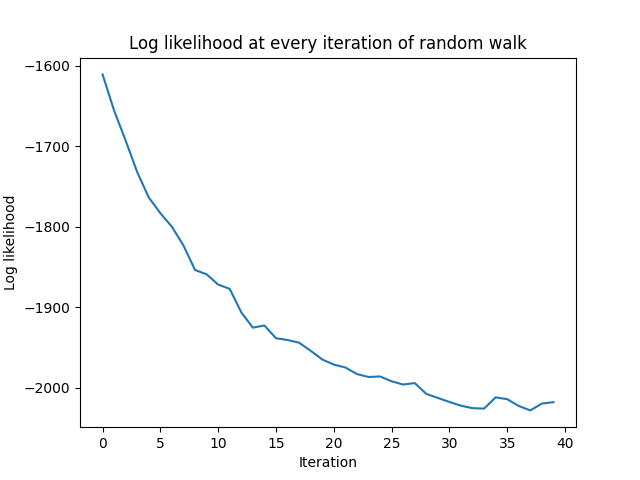
\includegraphics[width=1\linewidth]{dissertation/images/iterations_ll.png}
    \centering
    \caption{Average log likelihood of 10 trees with 20 taxa using random walk. At around iteration 15 of the random walk, there is no significant change in likelihood given further moves.}
\end{figure}

\subsubsection{SPR Network}

The network will use SPR move features inspired by Azouri's paper to predicting the likelihood improvement of said action. The features in particular that were chosen were:

\begin{itemize}
    \item Total length of the tree
    \item Total length of the subtree
    \item Total length of the regraft tree
    \item Distance between the subtree being moved and its relocation point
    \item The depth of the node being regrafted
    \item The depth of the point the node is being regrafted to
\end{itemize}

The output of the network is a prediction of the log likelihood increase that said move is likely to incur. This likelihood improvement is calculated with RAxML-NG. The prediction target can be calculated as

\[y\textsubscript{target} = l(x\textsubscript{i-1})- l(x\textsubscript{i}) \]

Where $x\textsubscript{i}$ is the tree at random walk iteration $i$, and $l(x)$ is the log likelihood function. To ensure the network can reliably differentiate desirable moves from undesirable ones, it is important to train on unbiased data. For this reason, the random walk for the SPR network includes the use of negative examples, or moves which decrease the log likelihood of the tree. The outputs of the network for each SPR move can then be compared, and the one which incurs the highest likelihood increase can be selected. 


\subsubsection{GNN Network}

The objective of the GNN is to predict which nodes are the most "out of place". That is, given a graph (phylogenetic tree), it finds the nodes which would lead to the highest likelihood improvement if the node was moved someplace else. The aim is to identify which nodes should be prioritized to be moved, instead of where to be moved. A node-level prediction will be performed on the input graph. Features are calculated via an amino acid distribution aggregation. To find the data per node, the aggregation method needs to take place starting at the leaf nodes working up to the root. At every node visited, the parents's amino acid distributions are calculated. Given there are a total of $2n-1$ nodes in a tree with $n$ taxa, the complexity of aggregating node data is of $O(n)$ time complexity. A graphic depiction can be found in Figure 5. The last data item that is included for each node is its depth: calculated as the number of nodes above it. The root node would have a depth of 0, and a leaf node with the most clades above would have the maximum depth.

Node features involving simple numeric totals were tested, as were features describing the potential subtree (similar to the SPR network). However, none were found to have the same efficacy and speed as the distribution method devised. 

\begin{figure}
    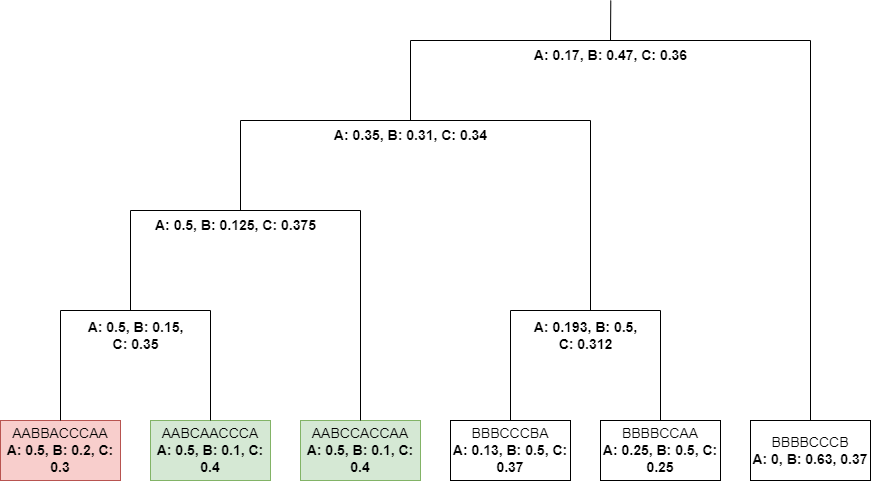
\includegraphics[width=1\linewidth]{dissertation/images/GNN_feature_generator.png}
    \centering
    \caption{An example of the amino acid distribution aggregation. At each connection (clade), the mean appearance of each amino acid of the two connecting clades is calculated.}
\end{figure}

After thorough testing of the random walk method, it was found that the neural network was not able to converge due to class imbalance. Therefore, an extra data generation tool was used for the GNN which we call multiple-move. Since at every move only 1 node was marked as incorrect, the dataset was saturated with nodes which should not be moved (therefore causing a class imbalance). To avoid this, several moves were done on a singular tree, with the opposite all marked as viable nodes to move. This form of data augmentation allowed for an increase in network accuracy, as it prevented the network from always predicting that the node should stay still. This was done by ensuring a more balanced distribution between nodes that are out-of-place and those that are not. This was done in conjunction with class re-weighing. A drawback of this design is it assumes that moves not performed are negative examples. We assume that the nodes that were not selected are going to be in place, that is, not out-of-place.

A ranking of the data was considered, wherein all the nodes would be ranked based on how "out-of-place" they are likely to be. However, this was found to be computationally unfeasible, as each possibility would need to be calculated by RAxML-NG. Given the runtime, using this method quickly became intractable.


\subsubsection{Node Network}

To ensure fair comparison with the GNN, each node had the exact same features as with the GNN. The multiple-move method was used to generate the training dataset, also to keep them the same. The only difference being the ratio of positive to negative instances of node movements. This was part of the data augmentation process, and was one of the main points of comparison to improve the node network. Apart from this, only the edge data was not included in the node network. It's worth noting that the node network data generation was significantly faster in generation time- as there was no need to build a PyTorch-compatible tree at every iteration. 


\subsection{Neural Networks}

Training data is used as described in section 3.2. Every network was built with Pytorch, and every network architecture was optimized manually over several iterations. Since there is very little similar previous work, a lot of the ideal network architectures had to be estimated and assumed.

\subsubsection{SPR Network}

Using the training data described in section 3.2.1, there were 6 inputs to the neural network. There are 2 hidden layers as shown in Figure 6, with only 1 output, the predicted log likelihood increase of the move. A mean squared loss function was used to assess the final value, following a standard optimization approach. The Adam optimizer was used to train the neural network \cite{kingma2014adam}. After hyperparameter tuning, the learning rate was set to 0.0001, batch size to 3, and the optimal number of epochs was 75, although early stopping was used.

\begin{figure}
    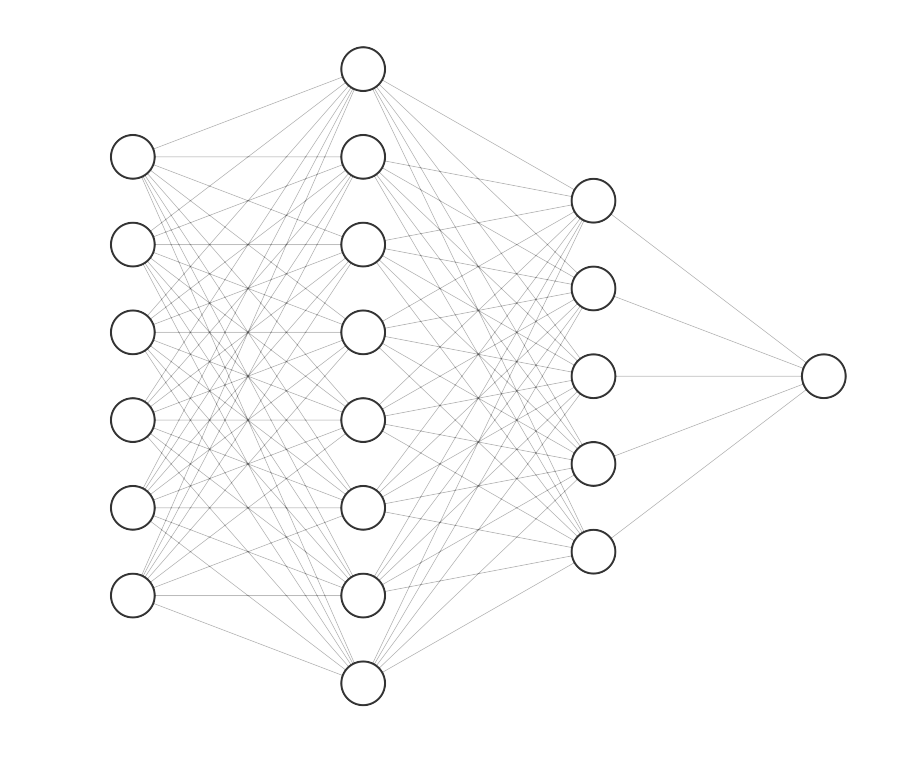
\includegraphics[width=1\linewidth]{dissertation/images/spr_nn.png}
    \centering
    \caption{A visualization of the SPR network: 6 inputs, 2 hidden layers, and 1 output.}
\end{figure}


\subsubsection{GNN}

Built by Pytorch Geometric \cite{fey2019fast}, the node-level GNN is actually a GCNN (Graph Convolutional Neural Network) and uses two graph convolutional layers followed by two linear layers. A visual representation of the convolutions can be found in Figure 7, and the convolution outputs are fed into a neural network identical to the node network, seen in Figure 8. Each graph node has two outputs: likelihood of being an "out-of-place" node, and the likelihood of not being out of place. A binary cross-entropy function is used as the loss function, trained with the Adam optimizer \cite{kingma2014adam}. The optimal hyperparameters found were: a learning rate of 0.0002 and the number of epochs being 70 (with early stopping). Depending on the training data used (random walk or multiple moves per graph) and the number of items in the dataset, the class weights are measured differently. As seen in section 3.2.2, using random walk gives an unbalanced dataset, and therefore re-weighing is required.

SiLU is used as the activation function between layers, and a dropout layer is employed after the convolutions as to prevent overfitting. Outputs from the GNN can be compared to find the most probable candidate for any given graph. This is done by finding the maximum value in the "out-of-place" probability output for each node.

\begin{figure}
    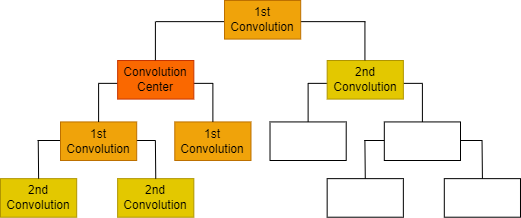
\includegraphics[width=1\linewidth]{dissertation/images/gcnn.png}
    \centering
    \caption{A visual representation of the graph convolution. Each rectangle in this diagram is a node (taxa or clade) containing features described in section 3.2.2}
\end{figure}


\subsubsection{Node Network}

The only difference in input between the node network and the GNN is the lack of neighbour information for the node network. Other than that, all input data remains the same. There are 22 inputs as there are 20 different amino acids in the dataset, 1 input for the ratio of empty amino acids, and 1 input for the depth of the node. There are 2 hidden layers in the node network, and there are 2 outputs (binary classifier). Figure 8 shows a graphic representation of the network. Binary cross-entropy loss with logits is used as a loss function, and the Adam optimizer \cite{kingma2014adam} employed to train the network. 

\begin{figure}
    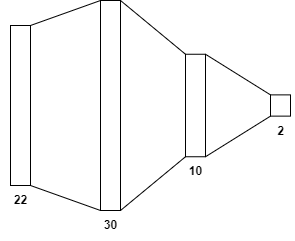
\includegraphics[width=1\linewidth]{dissertation/images/node_nn.png}
    \centering
    \caption{A visualization of the node network: 22 inputs, 2 hidden layers, and 2 outputs.}
\end{figure}

\vspace{10pt}

\subsection{Model Optimizations}

Optimizing the networks was an important part of the project. Early epoch stopping was used to find the maximum score, which was calculated in different ways depending on the network. The SPR network used the percentage of moves in top five as its main quality metric, and the GNN and node network used the balanced accuracy as its score metric. Balanced accuracy takes into account the class imbalance of the dataset, preventing bias to the majority class.

All networks went through batch size and learning rate optimizations, which were optimized via a 5-fold cross-validation method. Model architecture was optimized through trial and error, as well as general guidelines. Furthermore, both random walk and the multiple-move data generation method was tested on the GNN and node networks. Various data augmentation ratios were also tested with multiple move data generation on the node network and GNN. The results in section 4 are based on the optimal hyperparameters found during this tuning process.

\subsection{Final Algorithm}

Inspired by AlphaZero, the search algorithm will use a policy network and a value network. The policy network will be used to find the best nodes to move, and the value network will be used to score the SPR moves themselves. Since the main operation slowing down existing methods is the likelihood estimation, predicting the likelihood increase leads to a decrease in runtime. Figure 9 shows the policy and value network in action. The policy network will find which nodes need to move, and the value network will score the SPR moves from these nodes. The policy network in our paper can be either the GNN or the node network. Results in section 4.2 describe which was best at performing this task. The value network is the SPR network, which was inspired by Azouri's random forest algorithm. 

This method also allows for every node to be considered under an SPR move. Existing methods use local neighbour search to cut down the number of possible SPR moves. Local neighbour search is when an SPR move will only be considered with nodes that are at a certain proximity to the node being analyzed, allowing for a linearized complexity instead of a quadratic complexity. RAxML-NG uses a local neighbour search, for example. This drops the complexity of possible moves from $O(n^2)$ to $O(mn)$ such that $m$ is the average number of closest local neighbours set as a constant. A main drawback of this operation is that it cannot explore nodes which are further away, as they are not in the neighbourhood of nodes they should switch with. Using our method, all nodes can still be considered equally without compromising linear complexity. 

To join the networks together into a final search algorithm, a greedy search was devised. The policy network first scores each node by how "out-of-place" they are, and the ones with the highest value have their SPR move sets generated. Following this, the value network scores each SPR move. The highest SPR move from the set of possible moves is used as the next operation on the tree. This is continued iteratively until a maximum value is reached. Visually, Figure 10 shows the algorithm in terms of states and actions: a phylogenetic tree is the state, and an SPR move is the action.

Calculating the algorithmic complexity was done as follows: $O(n)$ complexity for calculating the node features, $O(1)$ complexity for both the policy and value networks, and $O(mn)$ such that there are $m$ top candidates for finding all the possible SPR moves. These can be joined together to form a complexity of $O(2mn*i)$ where $i$ is the number of iterations, as the node features and top candidate calculations are only performed once per iteration. Therefore, the time complexity of the algorithm is $O(n)$, or linear complexity. The memory complexity is of $O(n)$. This is because at each iteration, there is a fixed number of SPR moves and candidate nodes. This number depends on constants set by the program at the beginning of execution, and not by the number of sequences. However, the memory requirement is dependant on the number of sequences, as more memory will be needed for larger sets of sequences.

\begin{algorithm}
    \removelatexerror% Nullify \@latex@error

    \DontPrintSemicolon
    \KwData{Implementation of the search function, $search()$}
    \KwResult{A list of phylogenetic trees.}
    \Begin{
        $max\_depth \gets 30$\;
        $MSA \gets getPhylogeneticTree()$\;
        $current\_state \gets createUpgmaTree(MSA)$\;
        $best\_trees \gets [current\_state]$\;
        \While{$i < n\_iterations; i+1$} 
        {
            $actionSpace \gets getActionSpace(current\_state)$\;
            $bestSprMoves \gets policyNetwork(actionSpace)$\;
            $bestMove \gets bestSprMoves[0]$\;
            $bestMoveValue \gets 0$\;
            \For{$move \in bestSprMoves$}
            {
                $tempTree \gets current\_state.apply(move)$\;
                $tempTreeValue \gets valueFunction(tempTree)$\;
                \If{$tempTreeValue > bestMoveValue$}
                {
                    $bestMove \gets move$
                    $bestMoveValue \gets tempTreeValue$
                }
            }
            $current\_state \gets current\_state.apply(bestMove)$
            
            \If{$valueFunction(current\_state) > valueFunction(best\_trees[-1])$}
            {
                $best\_trees.append(current\_state)$
            }
        }
        \Return $best\_trees$
    }
\end{algorithm}


\begin{figure}
    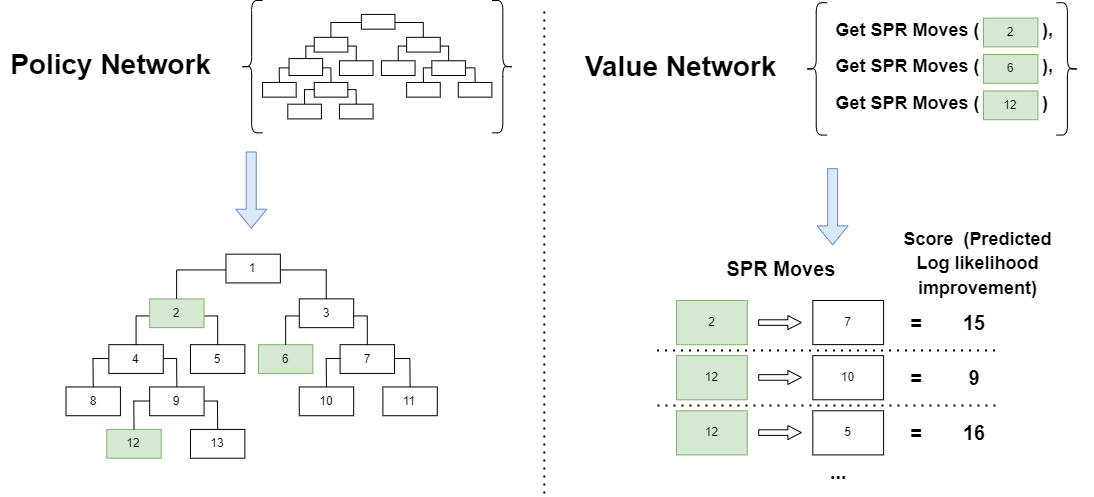
\includegraphics[width=1\linewidth]{dissertation/images/neural_algorithm.png}
    \centering
    \caption{The policy and value network in action. The policy network finds the most "out-of-place" nodes (highlighted in green). All possible SPR moves are calculated using said nodes, and the move features are fed to the value network, which gives a score for each.}
\end{figure}


\begin{figure}
    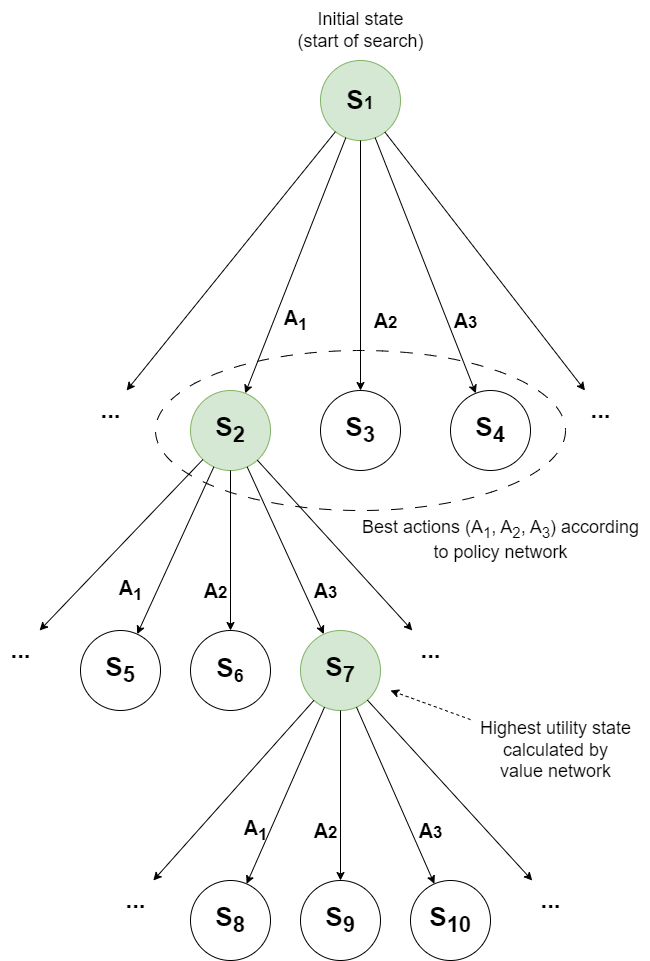
\includegraphics[width=0.8\linewidth]{dissertation/images/algorithm_in_action.png}
    \centering
    \caption{A visualization of the search for the best phylogenetic tree. Each state is a phylogenetic tree, and each action is an SPR move.}
\end{figure}


\subsection{Summary}

First, general assumptions involving the use of GNNs being suitable to find "out-of-place" nodes and the likelihood of the phylogenetic models remaining constant were stated. We then covered the generation of the training data, which used two methods: random walk for the value (SPR) network, and multiple-move for the GNN and node networks. The SPR network was trained to find the likelihood increase of an SPR move, which uses the features found in Azouri's paper. The GNN and node networks used an amino acid distribution aggregation function as features for each node. These were found using multiple-move, which is a method that randomly SPR moves several subtrees in a single tree, and sets all the reverse moves (and therefore nodes in the tree one move away) as potential candidates. The main advantage of multiple-move being an augmentation of the dataset, as random walk would have one move per tree instead of several.

Details of the neural network were then addressed, including the structure for the SPR and node networks (both using linear hidden layers with SiLU functions), and the GNN which used several convolutional layers followed by linear ones. All networks used the Adam optimizer to train the networks. The SPR network used MSE as its loss function, whilst the node network and GNN used binary cross-entropy loss, as the out-of-place node choice was defined as a binary classification problem. All networks were subject to manual and grid search hyperparameter optimization.

Lastly, the algorithm as a whole is discussed. The algorithm uses the output of the policy network to decide which nodes will move. Once these nodes have been identified, all possible SPR moves are calculated given the nodes. The SPR features are calculated, and fed into the SPR model, which scores them. The highest ranking SPR move is then selected as the next move the algorithm should take, and is executed. This continues for several iterations, until the program ends. The complexity is $O(n)$ and $O(n)$ for time and memory respectively.


\section{Evaluation}

To provide fair experimentation, all code to give results was run on the same ubuntu linux machine. RAxML-NG was installed on the machine, and the specifications were as follows: 
\begin{itemize}
    \item Intel(R) Core(TM) i9-10900X CPU @ 3.70GHz
    \item 131 GB of RAM
    \item Ubutu 22.04 LTS "Jammy Jellyfish"
\end{itemize}

\subsection{SPR Network}

The main test used to deduce the efficacy of the SPR network was a top 5 candidacy. Inspired by Azouri, it consists of checking whether the top SPR moves predicted are within the top 5 best likelihood improvements as calculated by RAxML-NG. Since the algorithm operates by checking the top candidates, it stands to reason that the more higher-value top-5 candidates are used, the better the algorithm will fare. Another simple metric used to assess the algorithm quality was loss: since it is trying to estimate a value, the less loss there is for unseen data, the better its ability to predict SPR values.

The average top 5 candidacy was found to be $22\pm 0.59 \%$ given the best trained model. We ran 10 trainings to get the mean and standard deviation of the top 5 candidate accuracy. This test was performed on unseen trees with 20 taxa per tree. Given that there are $(2n-1)^2$ SPR moves in a given tree and $n=20$, there are 1521 different possible SPR moves. A random algorithm would have a top 5 candidacy of on average $5/1521 = ~0.33\%$. A null hypothesis to test this network could be: The SPR network has a mean top 5 candidacy equal to the random algorithm. Given an alpha p-value of 0.05 for significance, we can test to reject the null hypothesis, which it does with a p-value $< 0.0001$ (extremely statistically significant).

The average loss on unseen datasets was quite high, and found to be approximately 7174. Mean squared loss was used to find these values, indicating that there is on average a difference of 85 between the prediction and the true value. The true values had a spread between -93 and 117, and a mean of 11.1. A loss value of this magnitude indicates that the network was likely able to discern whether an SPR move would bring a negative or positive change, but was not able to predict the likelihood increase precisely. This is evidenced by the top 5 candidacy metric, which showed that the network was able to choose the best moves.


\subsection{GNN and Node Network}

To compare the GNN and the node network, they were given the exact same training data. However, due to the nature of the GNN, it had access to neighbour node information, while the neural network did not. Furthermore, the node network data was easier to augment, as it is easier to remove instances from a node-to-classification dataset than it is a phylogenetic tree. For the sake of comparison, no data augmentation was performed on the cross validation. However it was used during optimization and best balanced accuracy results. 

\begin{figure}
    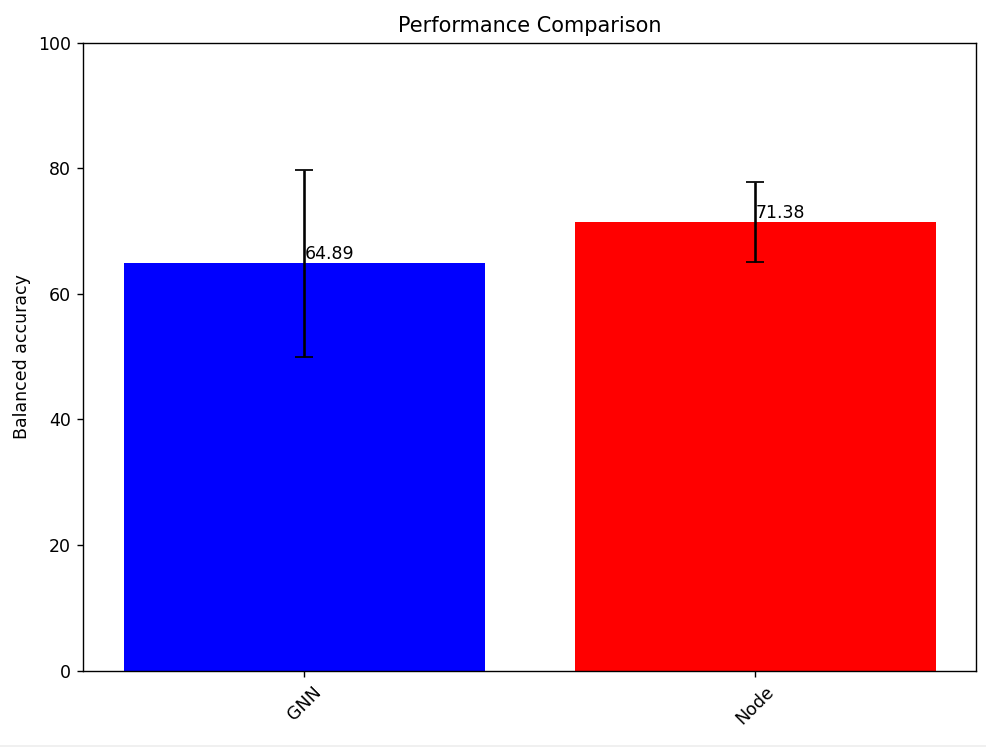
\includegraphics[width=1\linewidth]{dissertation/images/gnn_node_performance_comparison.png}
    \centering
    \caption{A 5-way cross validation balanced accuracy comparison between the GNN and the node network (no data augmentation). It can be seen in this graph that the node network was more effective at finding misplaced nodes. The error bars are standard error values.}
\end{figure}

Balanced accuracy was used to measure the quality of the neural networks. It is a metric which takes into account class imbalance by weighing the accuracy of false positives and true negatives. The top balanced accuracy found after hyperparameter optimization by the GNN was 81.34\%, and 79.45\% for the node network (which used data augmentation for this accuracy). The mean balanced accuracy for the GNN was 64.89 versus 71.38 for the node network as seen in Figure 11. It demonstrates that on average, the balanced accuracy of the node network is better than the GNN, and has less of an error range. In contrast, the GNN had a higher variety of balanced accuracy metrics. This implies that the GNN had a harder time converging on an accurate value, whilst the node network tended to be more stable. 

The average AUC score for the node network was 81\%, greatly outperforming the average AUC score for the GNN of 55\%. This is a good result, as 81\% is quite high. The GNN's average score is quite close to base randomness of 50\%, and is a poor result. The AUC result implies that the node network on average has a better performance than the GNN.

Upon closer inspection of the GNNs, it was noticed that the higher scoring models tended to highly attenuate or completely ignore the neighbour node information. This is an interesting result as it could imply that the neighbour data was not useful and did not add any new information. However, it could also be that there was not enough data or GPU time to allow the GNN to converge and use neighbour data. Since the node network and GNN have the same topology (after the convolution for the GNN), it can be deduced that the highest-scoring GNNs simply disregarded the convolutions and fed the data directly to the linear network.

Random walk for the GNN was not feasible due to the imbalance it creates between nodes that need to be moved and nodes which do not need to be. Given 20 taxa, there are 39 possible nodes to move, and therefore there is a ratio of $(2n-1):1$ given $n$ taxa. For any reasonably sized tree, this method is not possible for the GNN, as the class imbalance prevents conversion of the neural network. For this reason, only multiple-move could be used to train the GNN. In contrast, the node network could use random walk, and with data augmentation the abundant class could be cut down to a more manageable but still realistic 5:1 ratio.

\subsection{Algorithm}

To test our algorithm, there were multiple metrics to experiment with. We ran testing over 10 new unseen trees (generated by ROSE and RAxML-NG), and not those that the neural network trained with. RAxML-NG's model optimization parameter was turned off, as optimizing LG's parameters would make for an unfair experiment. This is because, as mentioned in section 3.1, we kept the amino acid model parameters constant. Furthermore, due to the results found in section 4.2, it was decided that the node network would be used in the algorithm to maximise its potential. 

\begin{figure}
    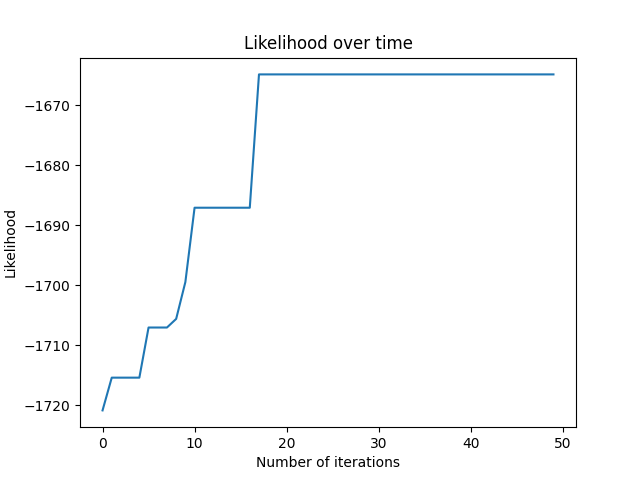
\includegraphics[width=1\linewidth]{dissertation/images/alg_output.png}
    \centering
    \caption{An example output of our algorithm running. The output is the maximum log likelihood found while the algorithm was running at every iteration. For this tree, RAxML-NG found a max log likelihood of approximately -1401, whilst our algorithm found a value of approximately -1667.}
\end{figure}

The experiment was run on several trees, and one of them was graphed as can be seen in Figure 12. The graph showcases the maximum log likelihood found over time, and although it does increase, it does not reach the same result as RAxML-NG.

\begin{figure}
    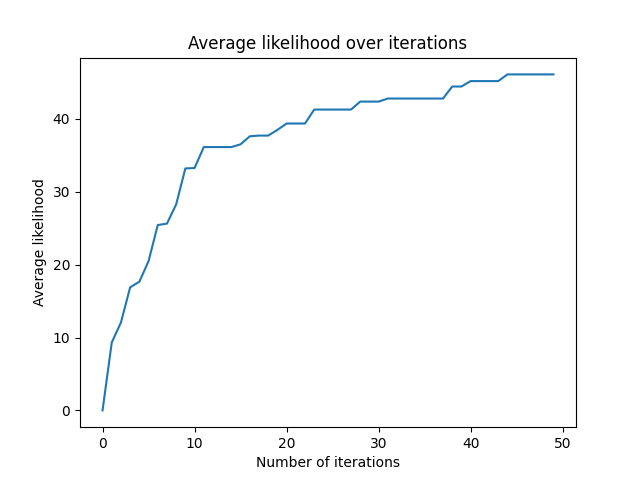
\includegraphics[width=1\linewidth]{dissertation/images/average_likelihood_improvement.png}
    \centering
    \caption{The average log likelihood improvement average on 10 trees after 50 iterations.}
\end{figure}

After running on 20 unseen trees with each 20 taxa, the log likelihood and timing values found on RAxML-NG and our algorithm were:

\begin{itemize}
    \item RAxML-NG average final likelihood was -1571.58
    \item Our algorithm's average final likelihood after 50 iterations was -1855.30
\end{itemize}

The average log likelihood improvement at each iteration for every tree was also calculated and graphed in Figure 13. This graph is informative in that it shows the average likelihood increase that can be expected on a starting phylogenetic tree, and that the algorithm does on average increase the likelihood.

The next metric to be tested was the average runtime of both algorithms. The experiment was run on 50 iterations of our algorithm, with the RAxML-NG parameters set to default. For a dataset with 20 taxa, our algorithm had an average run time of 1.06 seconds, whilst RAxML-NG had a runtime of 0.26 seconds. However, when run with the number of taxa being 500, RAxML-NG took 174.78 seconds, and our algorithm took 64 seconds. A caveat to these results is the performance of our algorithm with the larger dataset: RAxML-NG found a log likelihood of -85369.9, and our algorithm found one of -94074.8. 

In the dataset with 20 taxa, RAxML-NG found a maximum likelihood of -1571.58 whilst our algorithm found \mbox{-1855.30}, meaning there is on average an 18\% decrease in log likelihood. For the larger dataset, there was an average decrease in log likelihood of 10\% compared to RAxML-NG. Furthermore, the runtime of our algorithm scaled linearly, unlike RAxML-NG. 

\subsection{Discussion}

\subsubsection{SPR Network}

Although the SPR network was utilized by the algorithm to increase the average log likelihood of phylogenetic trees, its performance remains questionable. The p-value found with regards to the top 5 candidacy metric was significant compared to random. However, a best result of 22\% is not all that high. Since phylogenetic trees are very sensitive to SPR moves, a wrong move could send it in the wrong direction and drastically reduce the likelihood potential of the tree. Compared to Azouri's random forest method, it is a long way from the 99\% found. It is debatable however if Azouri's paper is a fair comparison: they used a different dataset, and did not use a standard benchmarking tool such as Rose. 

Although the loss was found to be quite high, with an average error of 85, the top 5 candidacy shows us that the network was still able to find some of the best moves. The fact that there was a large spread in likelihood change values suggests that the network could accurately predict whether a move would be a net positive or a net negative. Closer analysis of the dataset revealed that a majority of moves are negative: that is, they make the tree likelihood worse. This reinforces the idea that the network could tell good and bad moves apart. However, it also implies that it cannot find the optimal move at every iteration, as it would need increased precision to differentiate the best positive SPR move.

Although the SPR network was not able to find the best SPR move with similar accuracy to Azouri's, it was still able to find top candidates. Furthermore, when used in the algorithm, it was able to increase the net likelihood of the tree. The fact that the network was able to achieve this suggests that neural networks for likelihood prediction is a viable approach to phylogenetic tree construction.

\subsubsection{GNN and Node Network}

Although one of the hypotheses of this research was that a GNN would perform well for this sort of task, we have demonstrated that our network did not perform better than a network without graph convolutions. The node network performed better than the GNN in almost every way, and was used in the algorithm to find better results. This finding is encouraged by the fact that higher scoring GNNs resorted to ignoring neighbour to get to a higher score. One major exception was an outlier where the GNN scored better than the node network. This may have been due to random chance, as we were not able to reproduce this result consistently. What is clear is that the amino acid distributions used as a feature to differentiate nodes was successful. Since the node network performed statistically significantly better than random, they are viable features as the networks were able to use them to decide which nodes were out-of-place. More experimentation would need to be performed to explore the efficacy of alternative node features.

Ignoring the neighbours could be due to a multitude of reasons. One potential explanation is that clades depend on the distributions of their children, and so perhaps the first convolution does not give any new information to the GNN. If connections had only been made between sibling nodes, maybe this could have given more useful information to the network. There is also the possibility of there not being enough data or GPU time to converge. More training time with varied datasets may lead to a better convergence and use of neighbour data.

The fact that the GNN had a wider range of balanced accuracy measures whilst the node network was more consistent reinforces this conclusion. Some potential reasons for the wider range of GNN accuracy values is the difficulty in converging on larger sets of parameters, and the idea that the convolutions do not give much more new information (as they are formed via child nodes). If the GNN learns to ignore the neighbour features, it seems it is able to get a higher accuracy, sometimes comparable to the node network.

The balanced accuracy of the average node network found is quite good, as 71.38\% is better than a random balanced accuracy of 50\%. Null hypothesis: the node network has a balanced accuracy close to 50\%. Conducting a t-test, the significance of this  result is p < 0.0001, rejecting the null hypothesis. There is a lot of room for improvement, however this result suggests that a correct node to move can be found. 


\subsubsection{Algorithm}

One of the main goals of the paper was to reduce the time taken to find phylogenetic trees without compromising accuracy. This goal was partially reached: the time taken to find a tree scales better than RAxML-NG. This was proven in section 3.5 to be the case as we have a $O(n)$ time complexity, compared to at least $O(n\sqrt{n} \log{(n)}) $ complexity for RAxML-NG with the LG model. Although the time taken for smaller datasets was larger with our algorithm, this can mostly be put down as slowdowns due to sub-optimal programming. Since the code in this research used python and other experimental packages, there are a lot of technical improvements to be done.

Though one goal was reached, another was not: the likelihood improvement of the algorithm did not do as well as RAxML-NG. The neural networks did not perform optimally, and have a lot of room for improvement. To further improve these networks, either more data or more GPU time is needed, followed by further optimizations in the neural layout of those networks.

It is important to note that the differences between node distributions in the tree become smaller as the size of the tree increases. Since both the GNN and node network use those distributions, it affects both equally. It may be important to mitigate this in some way by using a different data generation method, or finding a way to differentiate very similar distributions. However, the algorithm was still able to increase log likelihood of larger trees, implying that the magnitude of difference was enough between sub-branches further away.

A drawback of the multiple-move method was the assumption that any node not used in multiple move was not an out-of-place node. This is most likely not true: there are likely to be out-of-place nodes which were not used in multiple-move. An improvement to this algorithm (which was unfeasible due to computational constraints) would be ranking each node by how out-of-place they are. Furthermore, a node may be out-of-place but might not have any good SPR move, whilst another node may be less out-of-place but have a lot more viable SPR moves. Again, this could be solved by using a ranking instead of multiple-move.

That being said, the average increase in log likelihood demonstrate that using neural networks for node prediction is a viable approach. 


\subsubsection{Final Thoughts}

Although the algorithm is faster, it is not as accurate as other existing methods. The main problems facing this method is a lack of data and GPU time. Whilst the data is generated synthetically, it is nonetheless difficult to obtain as it requires a lot of processing power, mostly due to the number of times RAxML-NG is run. The data generation process took a long time, and therefore training on larger datasets would require not only a better GPU, but also more CPUs. As for GPU time, this goes for any neural network: the more training, the better the results will be.

Another potential improvement could have been the use of more descriptive node features. Although several types were tested, it remains to be seen if other node features could be more informative, especially with regards to the GNN and neighbour information. As the size of the tree increases, the differences between node amino acid distributions get smaller. This may impact the efficacy of the GNN and node network for larger trees. That being said, since the algorithm can compare SPR moves across the entire tree, the small differences in amino acid distributions may not matter. For other algorithms, a radial SPR move (one which is limited to close neighbours) is used to limit possibilities. With our algorithm, nodes from across the entire tree can be compared. Nodes further out in the tree are more likely to have drastically different amino acid distributions, thereby eliminating the problem.


\subsection{Summary}

The best SPR network was found to have a top 5 candidacy (a method of testing how many top SPR moves were found out of the real top 5) of 22\%. Results between the GNN and node network were also compared, and the node network was found to have a better overall average performance with 71.38\% balanced accuracy compared to 64.89\% for the best GNN. The best scoring GNNs were also found to ignore neighbours, and had a wider range of accuracy values. The algorithm was tested as a whole, and was found to scale significantly better than RAxML-NG. However, log likelihood improvement was not comparable, with our algorithm achieving a log likelihood that was significantly less than RAxML-NG. The final thoughts discussed the need for more data, which is difficult to obtain as it takes a long time to process, and the need for more GPU time. Overall, the algorithm was found to have some positive and negative aspects, with a lot of room for improvement. But most importantly, it is most likely a viable method of phylogenetic tree construction.

\section{Conclusions}

\subsection{Conclusion}

Phylogenetic trees are a way of clustering taxa using amino acid chains and their similarity. There are many different ways to construct these trees, from using algorithmic methods to deep learning. The most popular methods revolve around the use of maximum likelihood estimation. These methods estimate the likelihood of a tree forming given the amino acid data. The likelihood is maximised using SPR (Subtree Pruning and Regraft) moves to reorganise the tree. In this research, we focused on building neural networks to help us optimize this process. A value network, called the SPR network, was trained to predict the log likelihood improvement that an SPR move could give. This followed from Azouri et al's work \cite{azouri2023tree}, where they used a random forest model to predict the best SPR move given a set of them. There were then 2 policy networks which were trained and compared, a GNN and a node network. The GNN used graph convolutions, whilst the node network simply used features of each node on the phylogenetic tree. The node network was found to have on average a higher balanced accuracy, and was used in the final algorithm. The algorithm was able to perform fast, with $O(n)$ complexity, but was unable to do so without compromising log likelihood improvement, performing worse than RAxML-NG. However, there was still an increase in log likelihood improvement, and considering the linear time complexity, there is a lot of room for improvement. 

\subsection{Future Work}

MCTS (Monte Carlo Tree Search) is a method which is used in the AlphaZero paper, and which was thought of in this experiment. The basic idea would be to implement training into the algorithm, and use the final log likelihood to re-train the neural networks based on decisions taken. This would add another layer of reinforcement learning, and could teach the neural networks to work in a way in which the output of the other is taken into consideration for the prediction.

Furthermore, there is work to be done on using different substitution models and their different parameters. As mentioned in section 2.5, only the LG model with default parameters is used to train the neural network. The choice of model and its parameters is important to the final log likelihood of the tree, and so finding a way to incorporate those parameters into training would be an important next step. One way to do this would be to use them as inputs for the neural network, but this would require a lot more training data, as you would need examples for each set of parameters.


\bibliographystyle{abbrv}

% \vspace{1}

\bibliography{citations}


\end{document}
